\section{红细胞网状模型}
\frame{\frametitle{网状模型和连续模型}
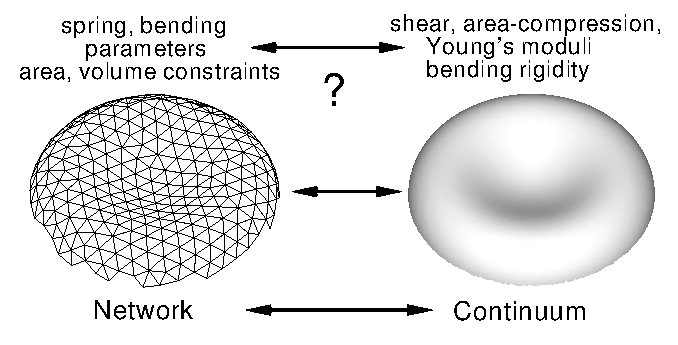
\includegraphics[width=\textwidth]{network2continuum.pdf}
}

\frame{\frametitle{网状模型和连续模型}
笛卡尔坐标系下的节点$\{\mathbf{x}_i\}, i\in 1\cdots N_v$构成二维三角形网络. 节点间由$N_s$个弹簧构成了$N_t$个三角形. 系统的势能
\[
V(\{\mathbf{X}_i\}) = V_{\text{in-plane}} + V_{\text{bending}} + V_{\text{area}} + V_{\text{volume}}
\]
每个节点的受力
\[
\mathbf{f}_i = -\frac{\partial V(\{\mathbf{x}_i\}) }{\partial \mathbf{x}_i}, \; i\in 1\cdots N_v
\]
}



\frame{\frametitle{面能$V_{\text{in-plane}}$}
膜上弹性能
\[
V_{\text{in-plane}}=\sum_{j\in1\cdots N_s}U_s(l_j)+\sum_{k\in1\cdots N_t} \frac{C_q}{A_k^q}
\]
其中$U_s$可以是$U_{WLC}$, $U_{FENE}$, $\cdots$
\[
U_{WLC}=\frac{K_BTl_m}{4p}\frac{3x^2-2x^3}{1-x}, \; U_{FENE}=-\frac{k_s}{2}l_m^2\log[1-x^2]
\]
其中$x=l/l_m\in(0,1)$, 由平衡时的势能最小可推得
\[
C_q^{WLC}=\frac{\sqrt{3}A_0^{q+1}k_BT(4x_0^2-9x_0+6)}{4pql_m(1-x_0)^2}, \;
C_q^{FENE}=\frac{\sqrt{3}A_0^{q+1}k_s}{q(1-x_0^2)}
\]
}


\frame{\frametitle{弯曲能$V_{\text{bending}}$}
由Helfrich模型得到弹性模弯曲的能量
\[
E_c= 8\pi k_c(1-R/R_0)^2+4\pi k_g
\]

网状模型中膜弯曲的势能
\[
V_{\text{bending}}=\sum_{j\in1\cdots N_s}k_b[1-\cos(\theta_j-\theta_0)]
=\frac{4\pi k_b}{\sqrt{3}}\bigg(1-\frac{R}{R_0}\bigg)^2
\]
由$E_c=V_{\text{bending}}$, 且$k_g=-4k_c/3$得
\[
k_b=\frac{2}{\sqrt{3}}k_c
\]
}



\frame{\frametitle{面积能$V_{\text{area}}$和体积能$V_{\text{volume}}$}
表面积和体积守恒的能量
\[
V_{\text{area}}=\frac{k_a(A-A_0^{tot})^2}{2A_0^{tot}} + \sum_{j\in1\cdots N_t}\frac{k_d(A_j-A_0)^2}{2A_0}
\]

\[
V_{\text{volume}}=\frac{k_v(V-V_0^{tot})}{2V_0^{tot}}
\]
}


\frame{\frametitle{对应参数的确定}
\begin{center}
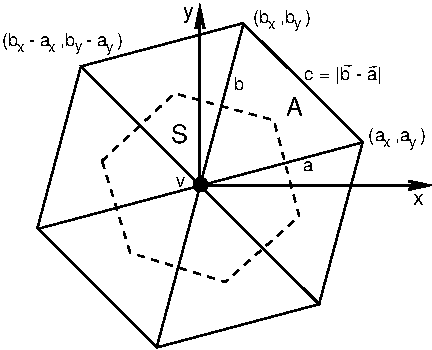
\includegraphics[width=0.8\textwidth]{hexagonalcell.pdf}
\end{center}
}

\frame{\frametitle{对应参数的确定}
在$V$节点周围$S=2A$的面积上的Cauchy应力
\begin{alignat*}{1}
\tau_{\alpha\beta} =& -\frac{1}{2A}\bigg[
\frac{f(a)}{a}a_\alpha a_\beta+\frac{f(b)}{b}b_\alpha b_\beta + \frac{f(c)}{c}c_\alpha b_\beta
\bigg]-\\
 & -\bigg(q\frac{C_q}{A^{q+1}}+\frac{k_a(A_0^{tot}-N_tA)}{A_0^{tot}}+\frac{k_d(A_0-A)}{A_0}\bigg)\delta_{\alpha\beta}
\end{alignat*}
剪切模量可由$\mu_0=\partial \tau_{xy}/\partial \gamma|_{\gamma=0}$($\gamma$是微小的剪切应变)得到
%\[
%\mu_0^{WLC}=\frac{\sqrt{3}k_BT}{4pl_mx_0}\bigg(\frac{3}{4(1-x_0)^2}-\frac{3}{4}+4x_0+\frac{x_0}{2(1-x_0)^3}\bigg)
%\]
\[
\mu_0^{FENE}=\frac{\sqrt{3}k_s}{4}\bigg( \frac{x_0^2}{(1-x_0^2)^2} + \frac{2}{1-x_0^2} \bigg)
\]
}


\frame{\frametitle{对应参数的确定}
面内压力
\[
P=-\frac{1}{2}(\tau_{xx}+\tau_{yy})=\frac{3lf(l)}{4A}+q\frac{C_q}{A^{q+1}} + \frac{(k_a+k_d)(A_0-A)}{A_0}
\]
由$K=-\frac{\partial P}{\partial\log(A)}\bigg|_{A=A_0}=-\frac{1}{2}\frac{\partial P}{\partial log(x)}\bigg|_{x=x_0}$得到抗压模量
\[
K^{FENE}= \frac{\sqrt{3}ks}{1-x_0^2}\bigg[q+1+\frac{x_0^2}{1-x_0^2}\bigg] + k_a + k_d
\]
如果取$q=1$, 由于$k_a+k_d\gg\mu_0 \Rightarrow K\gg\mu_0$, 二维膜的Young氏模量
\[
Y=\frac{4K\mu_0}{K+\mu_0},  Y\rightarrow 4\mu_0 \text{ if } K\rightarrow\infty
\]

}


\frame{\frametitle{粗粒化}
节点数$N_v$,边数(弹簧数)$N_s$及面数(三角形数)$N_t$满足
\[
N_v-N_s+N_t=2, N_s=3N_t/2 \Rightarrow N_t=2N_v-4
\]
则球面上均分$N_v$个节点时, 其平均二面角
\[
\cos(\theta)=1-\frac{1}{6}\bigg[6\Big(
\frac{R^2}{a^2}-\frac{1}{4}\Big)\bigg] \Rightarrow \theta_0=\cos^{-1}\bigg(\frac{\sqrt{3}(N_v-2)-5\pi}{\sqrt{3}(N_v-2)-3\pi}\bigg)
\]
球面表面积与边长及节点数间的关系
\[
A=N_t\cdot A_0 = (2N_v-4)\cdot \frac{\sqrt{3}l_0^2}{4}
\]
}

\frame{\frametitle{粗粒化}
粗粒化(coarse-graining)模型与标准(``fine'')模型参数的关系
\[
l_0^c = l_0^f\sqrt{\frac{N_v^f-2}{N_v^c-2}}, \,\,\,\, 
l_m^c = l_m^f\sqrt{\frac{N_v^f-2}{N_v^c-2}}, \,\,\,\, 
k_s^c=k_s^f(\text{FENE})
\]
}

